\section{Results}\label{sec:results}
Figures~\ref{fig:main} and~\ref{fig:finite} pair coverage with width; Appendix~\ref{app:displays} reports sample-size trends and diagnostics, and Appendix~\ref{app:complete} retains every completed method/setting cell.
\begin{figure}[t]
\centering
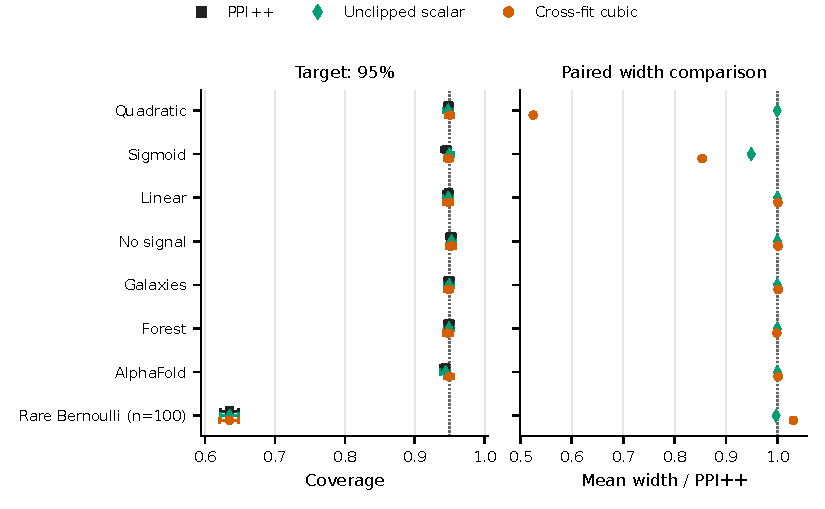
\includegraphics[width=\linewidth]{figures/main_comparison.pdf}
\caption{Nonlinear gains, no-gain controls, archive results and a small-sample failure. Scalar PPI++ (\texttt{ppi-python 0.2.3}), unrestricted scalar and cross-fitted cubic use identical inputs. All rows have $n=2000,N=20000$, except rare Bernoulli ($n=100,N=1000$); $R=5000$ repetitions per row. Left: coverage with 95\% Wilson Monte Carlo intervals. Right: ratios of paired mean widths to PPI++, with 95\% delta-method Monte Carlo intervals. Rare-event short intervals fail. The archive rows use independent with-replacement draws and target empirical archive means, with no broader population claim. These Wald intervals have asymptotic justification, not finite-sample guarantees.}
\label{fig:main}
\end{figure}
\paragraph{Nonlinear signal can leave substantial precision after scalar tuning.}
For quadratic Gaussian regression at $n=2000$, $N=20000$, the cubic/PPI++ ratio of mean widths is \QuadRatio{} (paired 95\% Monte Carlo interval \QuadRatioCI{}), a \QuadReduction{} reduction. Cubic coverage is \QuadCoverage{} (Wilson interval \QuadCoverageCI{}); PPI++ coverage is \QuadBaseCoverage{} (\QuadBaseCoverageCI{}). Both are compatible with the nominal target, while neither has an exact finite-sample guarantee. Against the unrestricted scalar, the ratio is \QuadUnclippedRatio{} (\QuadUnclippedRatioCI{}), so clipping is not the explanation. The predicted leading-order oracle ratio is $0.524$, closely matching the fitted result. Linear and no-signal cases instead give cubic/PPI++ ratios \LinearRatio{} and \NoSignalRatio{}, respectively, consistent with a small fitting cost and no first-order nonlinear benefit. These controls matter as much as the designed positive case.

\paragraph{Finite unlabeled information limits the gain.}
A documented follow-up after the initial real/bounded results repeats linear, quadratic and no-signal regimes with $n=N=2000$, using 3,000 repetitions. The quadratic ratio becomes \QuadEqualRatio{} (\QuadEqualRatioCI{}), close to the analytical prediction $0.775$, with cubic coverage \QuadEqualCoverage{} (\QuadEqualCoverageCI{}). The reduction from the $N=10n$ gain agrees with the second term in~\eqref{eq:optimum}; it does not establish performance at untested sample ratios.

\paragraph{Archived-data results show no practical nonlinear gain.}
At $n=2000$, cubic/PPI++ ratios are \GalaxyRatio{} (\GalaxyRatioCI{}) for galaxies, \ForestRatio{} (\ForestRatioCI{}) for forest, and \AlphaFoldRatio{} (\AlphaFoldRatioCI{}) for AlphaFold. Cubic coverage is \GalaxyCoverage{}, \ForestCoverage{}, and \AlphaFoldCoverage{}, respectively; their Wilson intervals include $.95$. The small forest reduction is approximately one tenth of one percent; the other two widen. At $n=500$ all three widen. These results concern the empirical distributions of archived labels and frozen predictions, with independent with-replacement draws. They support no claim of broader natural-population coverage or useful real-data shortening.

\paragraph{A narrow normal interval can fail badly.}
For rare Bernoulli outcomes with prevalence $.01$ and $n=100$, cubic coverage is \RareCoverage{} (\RareCoverageCI{}), label-only Wald coverage is \RareLabelCoverage{} (\RareLabelCoverageCI{}), and exact Clopper--Pearson coverage is \RareExactCoverage{} (\RareExactCoverageCI{}). The apparent Wald precision is inadmissible for the task's validity requirement. Zero-width intervals when all selected labels are zero remain in the summaries. The exploratory Holm-adjusted undercoverage diagnostic flags cubic intervals for galaxies and AlphaFold at $n=100$, and rare Bernoulli at $n=100,500$. Failure to reject in other cells is not a coverage certificate.

Cross-fitting also leaves nuisance-fit instability: at $n=100$, forest cubic widths have median $.131636$ and maximum $35.827096$, while AlphaFold has median $.101198$ and maximum $8.748830$. These large intervals are retained in means and uncertainty. Degree-12 and same-label plug-in diagnostics further expose fitting costs; they are not presented as automatically valid competitors.

\begin{figure}[t]
\centering
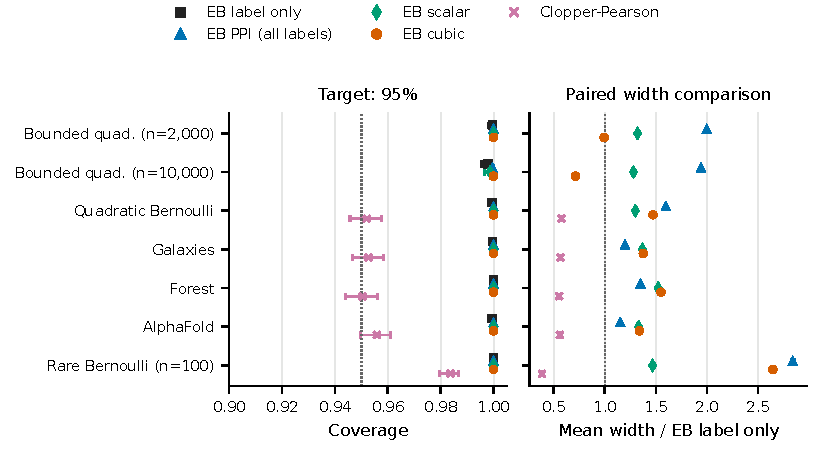
\includegraphics[width=\linewidth]{figures/finite_comparison.pdf}
\caption{Finite-sample guarantees can coexist with gains or substantial conservatism. EB methods have bounded-data guarantees under independent iid sampling; trained controls reserve labels from the original budget, while label/fixed-PPI baselines use all $n$. CP is exact binary label-only and is absent for nonbinary bounded rows. All rows have $n=2000,N=20000$, except labeled $n=10000$ bounded ($N=100000$) and $n=100$ rare-event ($N=1000$) rows. Bounded rows use $R=3000$; binary rows use $R=5000$. Left: empirical coverage with 95\% Wilson Monte Carlo intervals. Right: paired mean-width ratios to EB label-only with 95\% delta-method Monte Carlo intervals. The designed bounded case gains; archived empirical populations do not. These Monte Carlo intervals are distinct from target-mean intervals and theorem guarantees. This compares the stated EB/CP family.}
\label{fig:finite}
\end{figure}
\paragraph{Finite-sample guaranteed shortening is possible, but conservative.}
In the high-signal bounded-quadratic supplement, $n=10000$, $N=100000$, cubic EB/label-only EB mean-width ratio is \BoundedRatio{} (\BoundedRatioCI{}), a \BoundedReduction{} reduction. Against all-label unit-PPI EB it is \BoundedUnitRatio{} (\BoundedUnitRatioCI{}), and against trained scalar EB it is \BoundedScalarRatio{} (\BoundedScalarRatioCI{}). Cubic EB mean width is \BoundedWidth{} (Monte Carlo SE \BoundedWidthSE{}), and all 3,000 intervals cover (Wilson interval \BoundedCoverageCI{}). The $\ge95\%$ guarantee follows from boundedness and independent training, not this hit count. At $n=2000$, the ratio to label-only EB is \BoundedSmallRatio{} (\BoundedSmallRatioCI{}): range penalties nearly erase the gain.

On all three empirical populations, cubic EB is wider than label-only EB, all-label unit-PPI EB, scalar EB, and exact Clopper--Pearson. In the nonlinear Bernoulli case it can beat unit-PPI EB while losing to label-only EB and Clopper--Pearson. Thus the finite-sample success is limited to a designed high-signal setting and the measured EB comparator family. These conservative intervals also remain substantially wider than their Wald counterparts; comparing across guarantee classes cannot remove that cost.
